%!TEX root = ../../../../thesis.tex
\section{The Slime Mold Physarum Polycephalum}

	\Pp is an acellular slime mold belonging to the \emph{myxomycetes}\footnote{Myxomycetes, myxogastria or myxogastrea are all synonyms and denote a grouping of slime molds containing $5$ orders, $62$ genera and $888$ species~\cite{ainsworth2008ainsworth}.}. It is native to the forests of France, Italy, Spain, Romania, North-, Middle- and South America as well as China, Nepal, Southeast Asia and Japan. Its striking bright yellow renders the organism very noticeable, see \Fref{fig:exploration:forest}. In the recent past \P has become increasingly at home in research laboratories and schools across the globe where its extraordinary properties fascinate scientists and students alike, see \Fref{fig:exploration:lab}.

	\begin{figure}[!htp]
		\centering
		\subfloat[\P exploring the forest][]{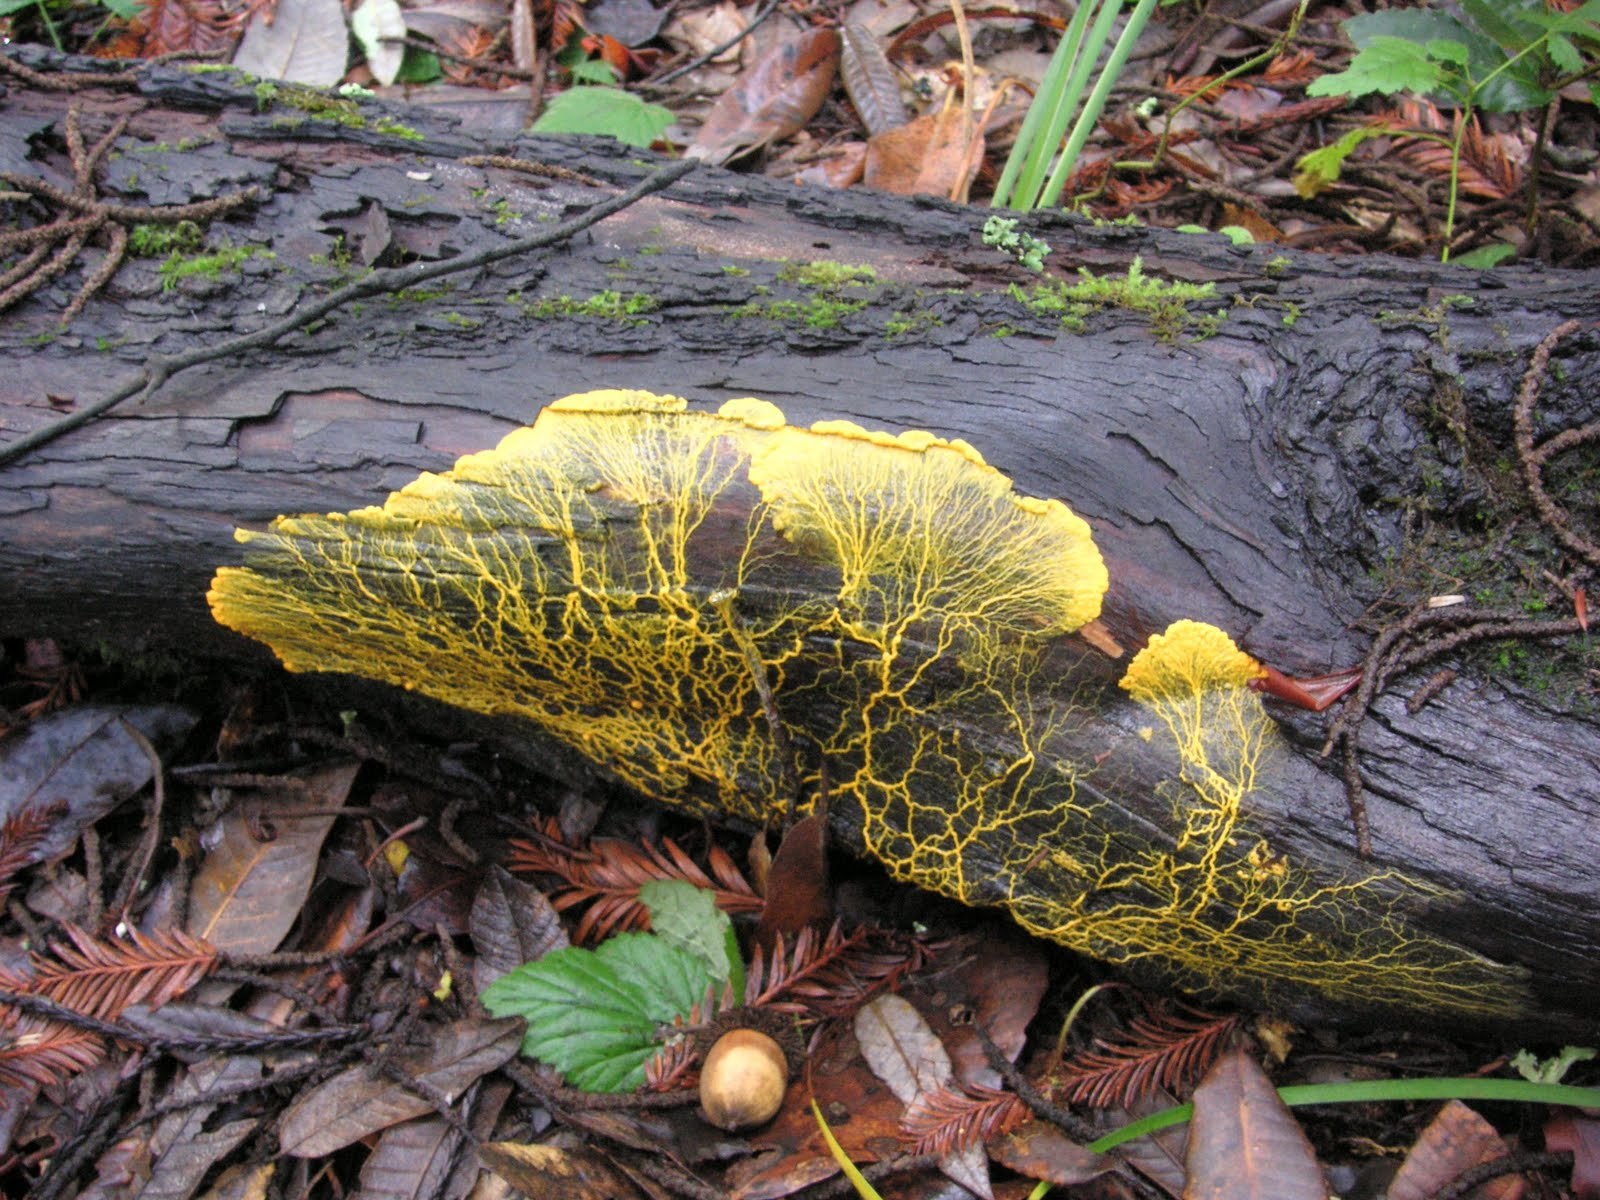
\includegraphics[width=\twoimageswide,keepaspectratio]{physarum_exploring_forest.jpg}\label{fig:exploration:forest}}
		\qquad
		\subfloat[\P exploring the lab][]{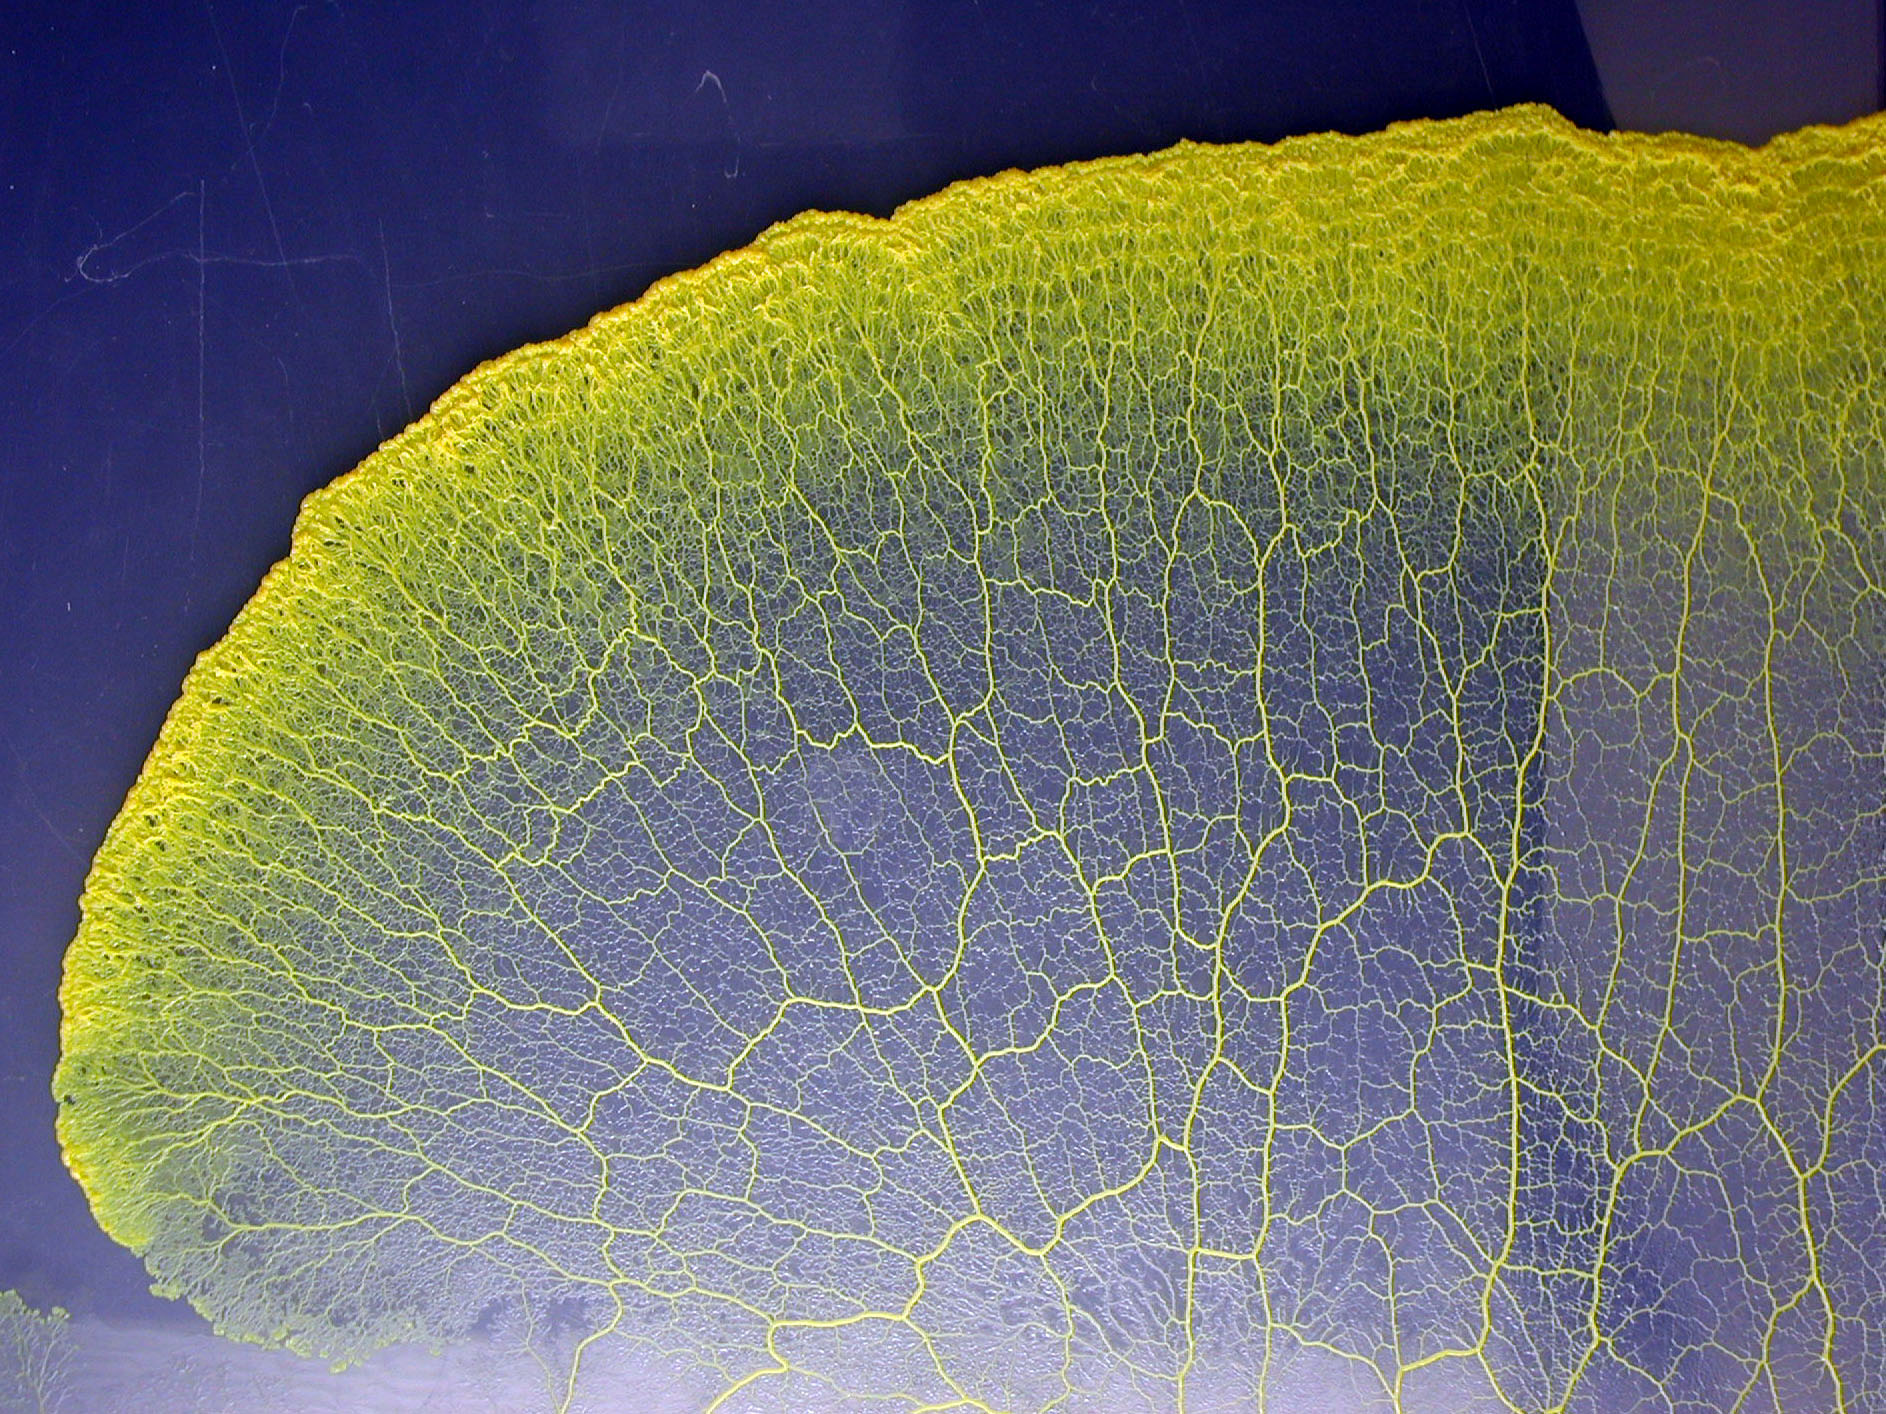
\includegraphics[width=\twoimageswide,keepaspectratio]{physarum_exploring_petri_dish.jpg}\label{fig:exploration:lab}}
		\caption[\P exploring various environments]{Today striking \P seems equally at home in the forest (a) and the in the laboratory (b). Figures courtesy of Prof.~T.~Ueda of Hokkaido University.}
		\label{fig:exploration}
	\end{figure}

	In the following we give a concise introduction to \Pp, discussing its life cycle and scientific importance. We emphasize the plasmodium stage in particular, which is of key importance for all natural computing applications discussed in \Fref{sec:natural_computing_physarum}. We summarize selected material from several sources which may be consulted for more detailed surveys~\cite{stephenson1994myxomycetes,nowotny2000myxomyceten,grube2016physarum,Sauer1986,Mayne2016,lifecycle}. Our exposition closely follows the structure of~\cite{nowotny2000myxomyceten}.
	
	\FloatBarrier
	
	\subsection{Life of Slime}


		The life cycle of \P starts with its spores which are propagated in a predominately airborne fashion. After an incubation period of a few days, spores begin to germinate given favorable conditions. In the process the walls of the spores break open to release haploid protoplasmic bodies of \SIrange{12}{15}{\micro\metre} in diameter. After a short period of quiescence these so-called myxoamoebae become active and start growing and multiplying much like other soil amoebae. 

		Two reversible processes illustrate the remarkable adaptability of \P myxoamoebae. First, they have the ability to quickly grow one or two flagellae, \ie change into myxoflagellates. This enables them to better navigate moist environments such as water films. If moist conditions are followed by dry ones, the organism can change back to its non-flagellate form. Second, both types of myxoamoebae may form dormant micro cysts capable of enduring adverse conditions such as extreme dryness or strong illumination. As soon as conditions become favorable again, myxoamoebae escape their cysts and are ready to continue the life cycle.

		In the next stage of the life cycle of \P, pairwise sexual or heterothallic fusion between two haploid myxoamoebae are observed. This leads to the irreversible formation of a diploid zygote. It is also possible that a single myxoamoeba changes directly into a haploid zygote in an apogamic or selfing fashion.

		Both types of zygotes have in common that from now on, nuclear division happens synchronously every \SIrange{8}{10}{\hour} without cell devision. This dramatic change signals the onset of a peculiar cellular organization, the so-called \emph{plasmodium}. In this stage \P lives as an macroscopic brightly yellow mass of protoplasm consisting of up to millions of nuclei contained in a singular cell. Remarkably, the plasmodium stage is unique to myxomycetes and unparalleled throughout all of nature.

		In its plasmodium stage \P is acting as an undifferentiated macroscopic creature, capable of sensing food sources, migrating towards them and feeding on them by means of phagozytosis. Typical food sources encountered by \P in the field include bacteria, amoebae, algae, common molds and various organic materials. It is also known to feed on spores, hyphen or fruiting bodies of fungi. In the lab \P can sustain itself on substrates containing solute nutrients. Under continued food intake, the plasmodium can grow to cover large areas of up to  several \si{\deci\metre\squared}. Under unfavorable conditions the plasmodium can change into many multi-nucleated dormant macrozysts, forming a crust of dried slime, the so-called \emph{sclerotium}. \P may reverse back to its plasmodium form in better conditions even after prolonged periods of lying dormant. 

		Towards the end of the life cycle, triggered by illumination, the plasmodium seeks out dry and preferably elevated locations to begin the irreversible process of sporulation. In a synchronous differentiation process \P forms colonies of \SIrange{1}{2}{\milli\metre} tall fruiting bodies. These so-called sporangia are numerous and come with a stem and a head each. Their appearance inspired its species designation \Pp, the multi-headed. Within the fruiting bodies, spores are maturing which are responsible for species propagation. After maturing, fruiting bodies break open allowing the contained spores to be dispersed by the wind. Thus the life cycle of \P, given suitable conditions, may start anew.

		It is fascinating how this multi-potent development system exists in extremely different forms of live while controlled by one and the same genome in a unique temporal sequence. From spores to amoeba, on to plasmodium and finally to fruiting bodies. From there back to spores and again into more amoeba. The complete life cycle of \Pp is illustrated in \Fref{fig:life_cycle}.

		\begin{figure}[htb]
			\centering
			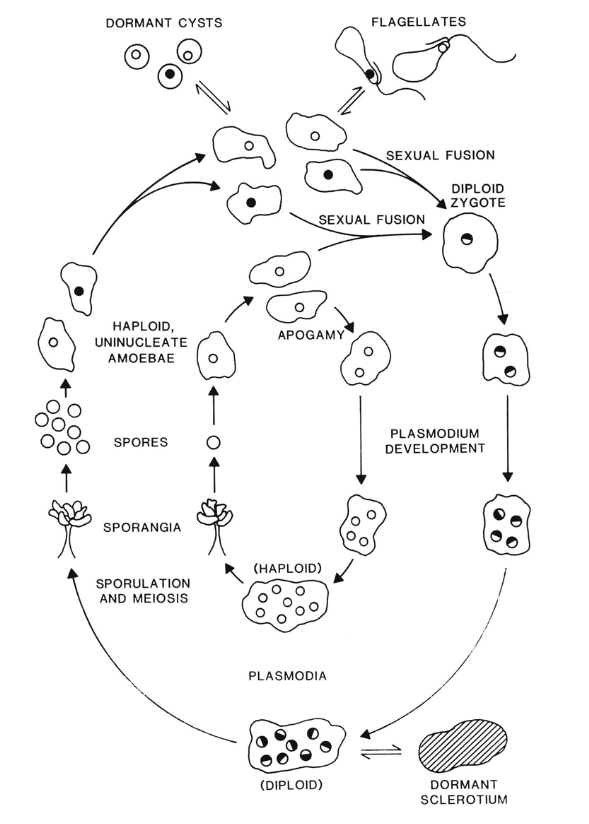
\includegraphics[width=\textwidth,height=0.8\textheight,keepaspectratio]{life_cycle.png}
			\caption[Life cycle of \P]{The complete life cycle of \Pp. Reprint from~\cite{Sauer1986}.}
			\label{fig:life_cycle}
		\end{figure}

		Next we discuss the plasmodium stage of \P in more detail as it is most relevant to this thesis.

		\FloatBarrier

	\subsection{The Plasmodium of P.~Polycephalum}

		The typical plasmodium of \P takes the shape of an extended sheet-like structure capable of moving to explore unvisited territory in search of food sources. \Fref{fig:exploration:lab} illustrates that in this stage of its life cycle, the organism consists of a complex vein network (bottom right area of image) which connects to the boundary of the organism, its apical zone or growing front (arcing from bottom left to top right). \Fref{fig:apical_zone} and \Fref{fig:supporting_network} show details of the apical zone and the vein network respectively. The overall shape of the network is highly dynamic and may change drastically in response to changing environmental conditions such as encountered attractants or repellents. This extraordinary functional plasticity allows \P to navigate its environment successfully.

		
		\begin{figure}[!htbp]
			\centering
			\subfloat[][]{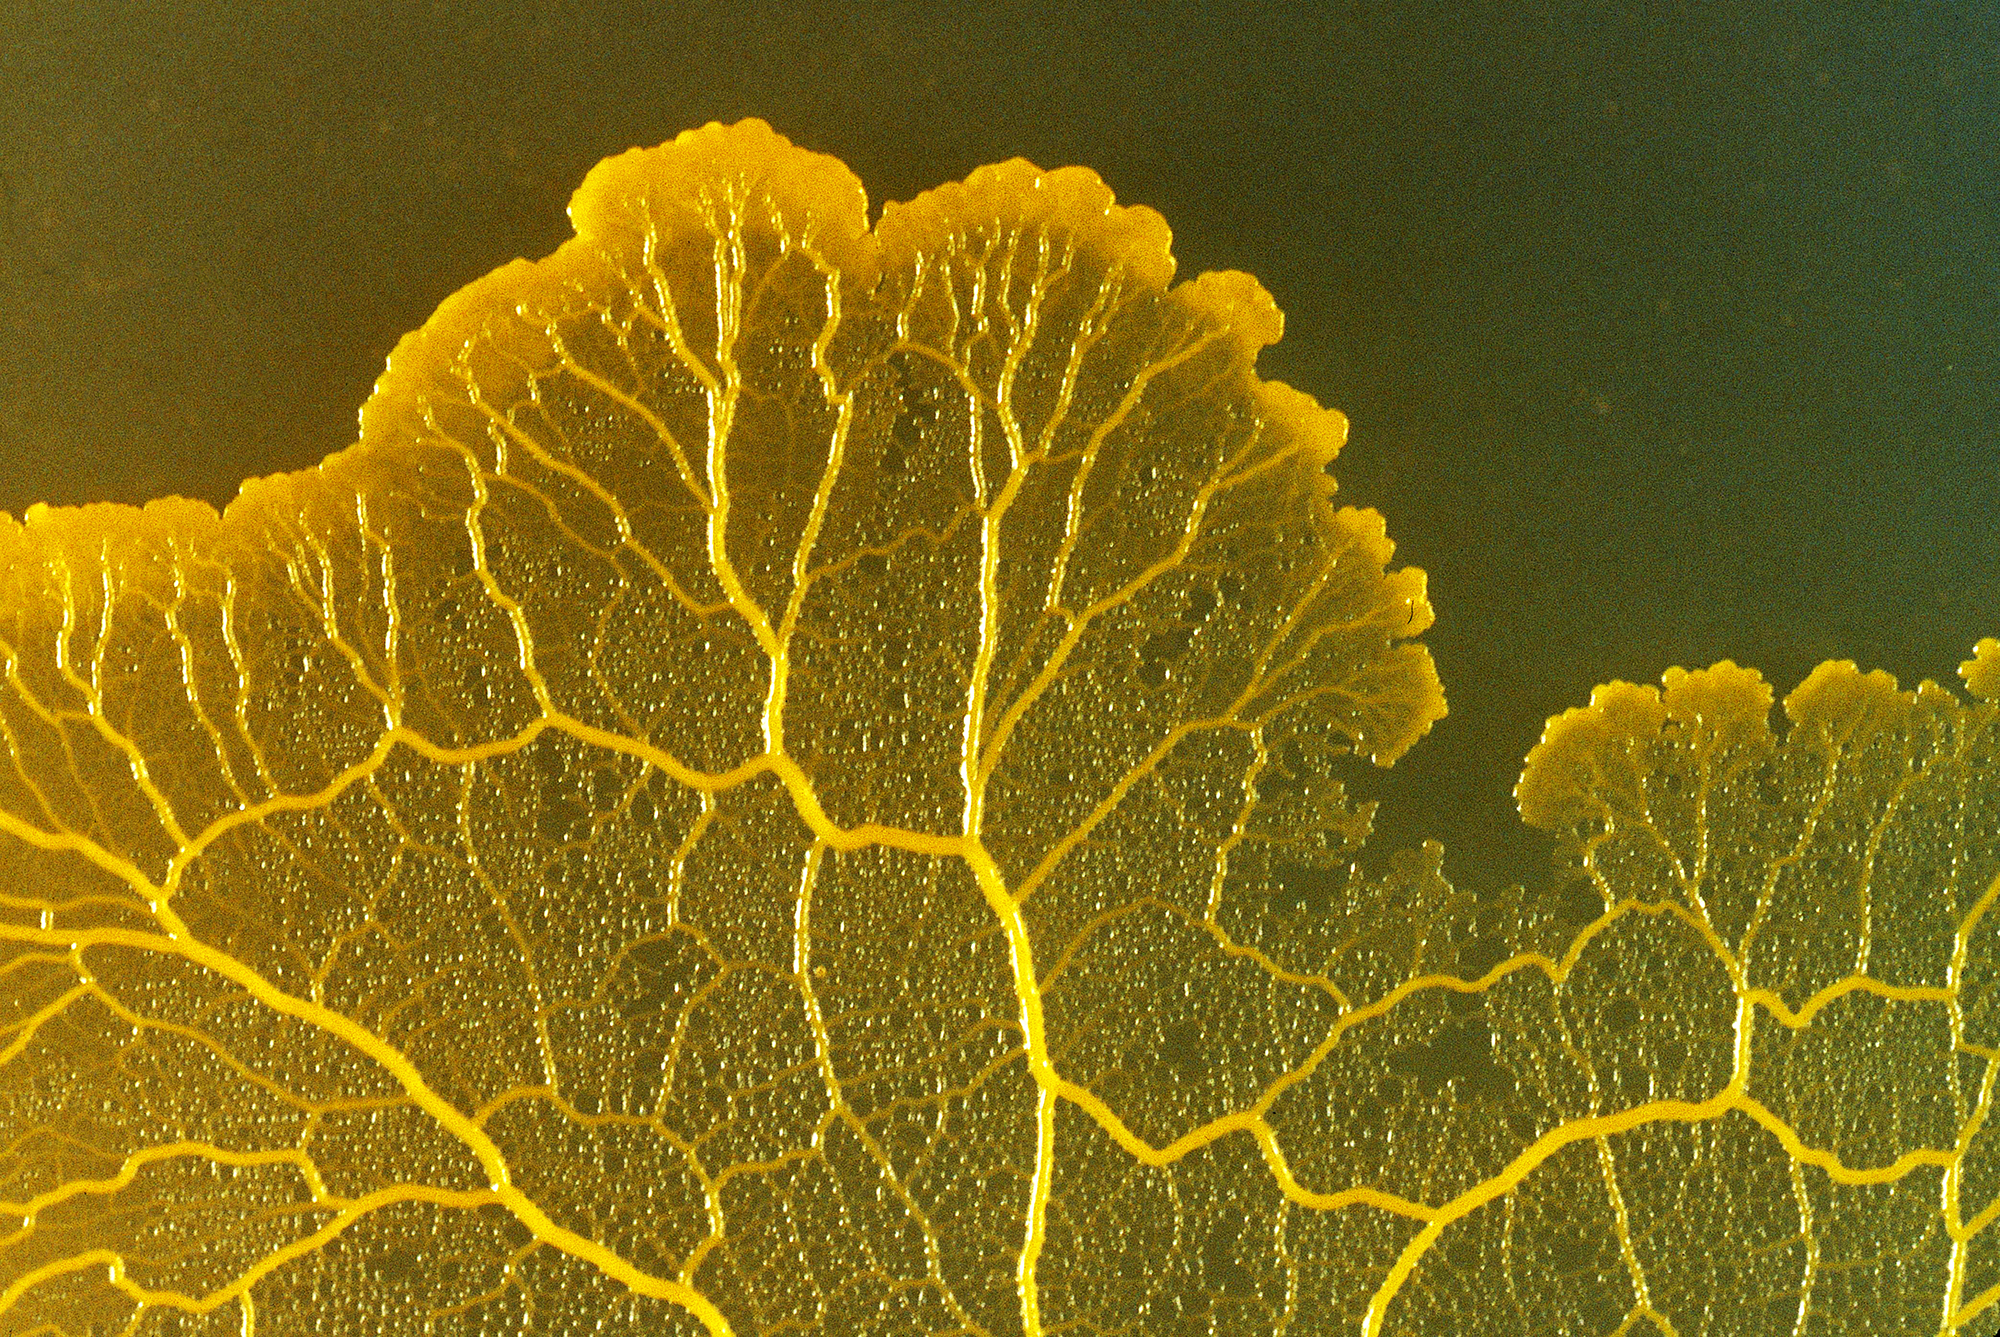
\includegraphics[width=\twoimageswide]{slime.jpg}\label{fig:apical_zone}}
			\qquad
			\subfloat[][]{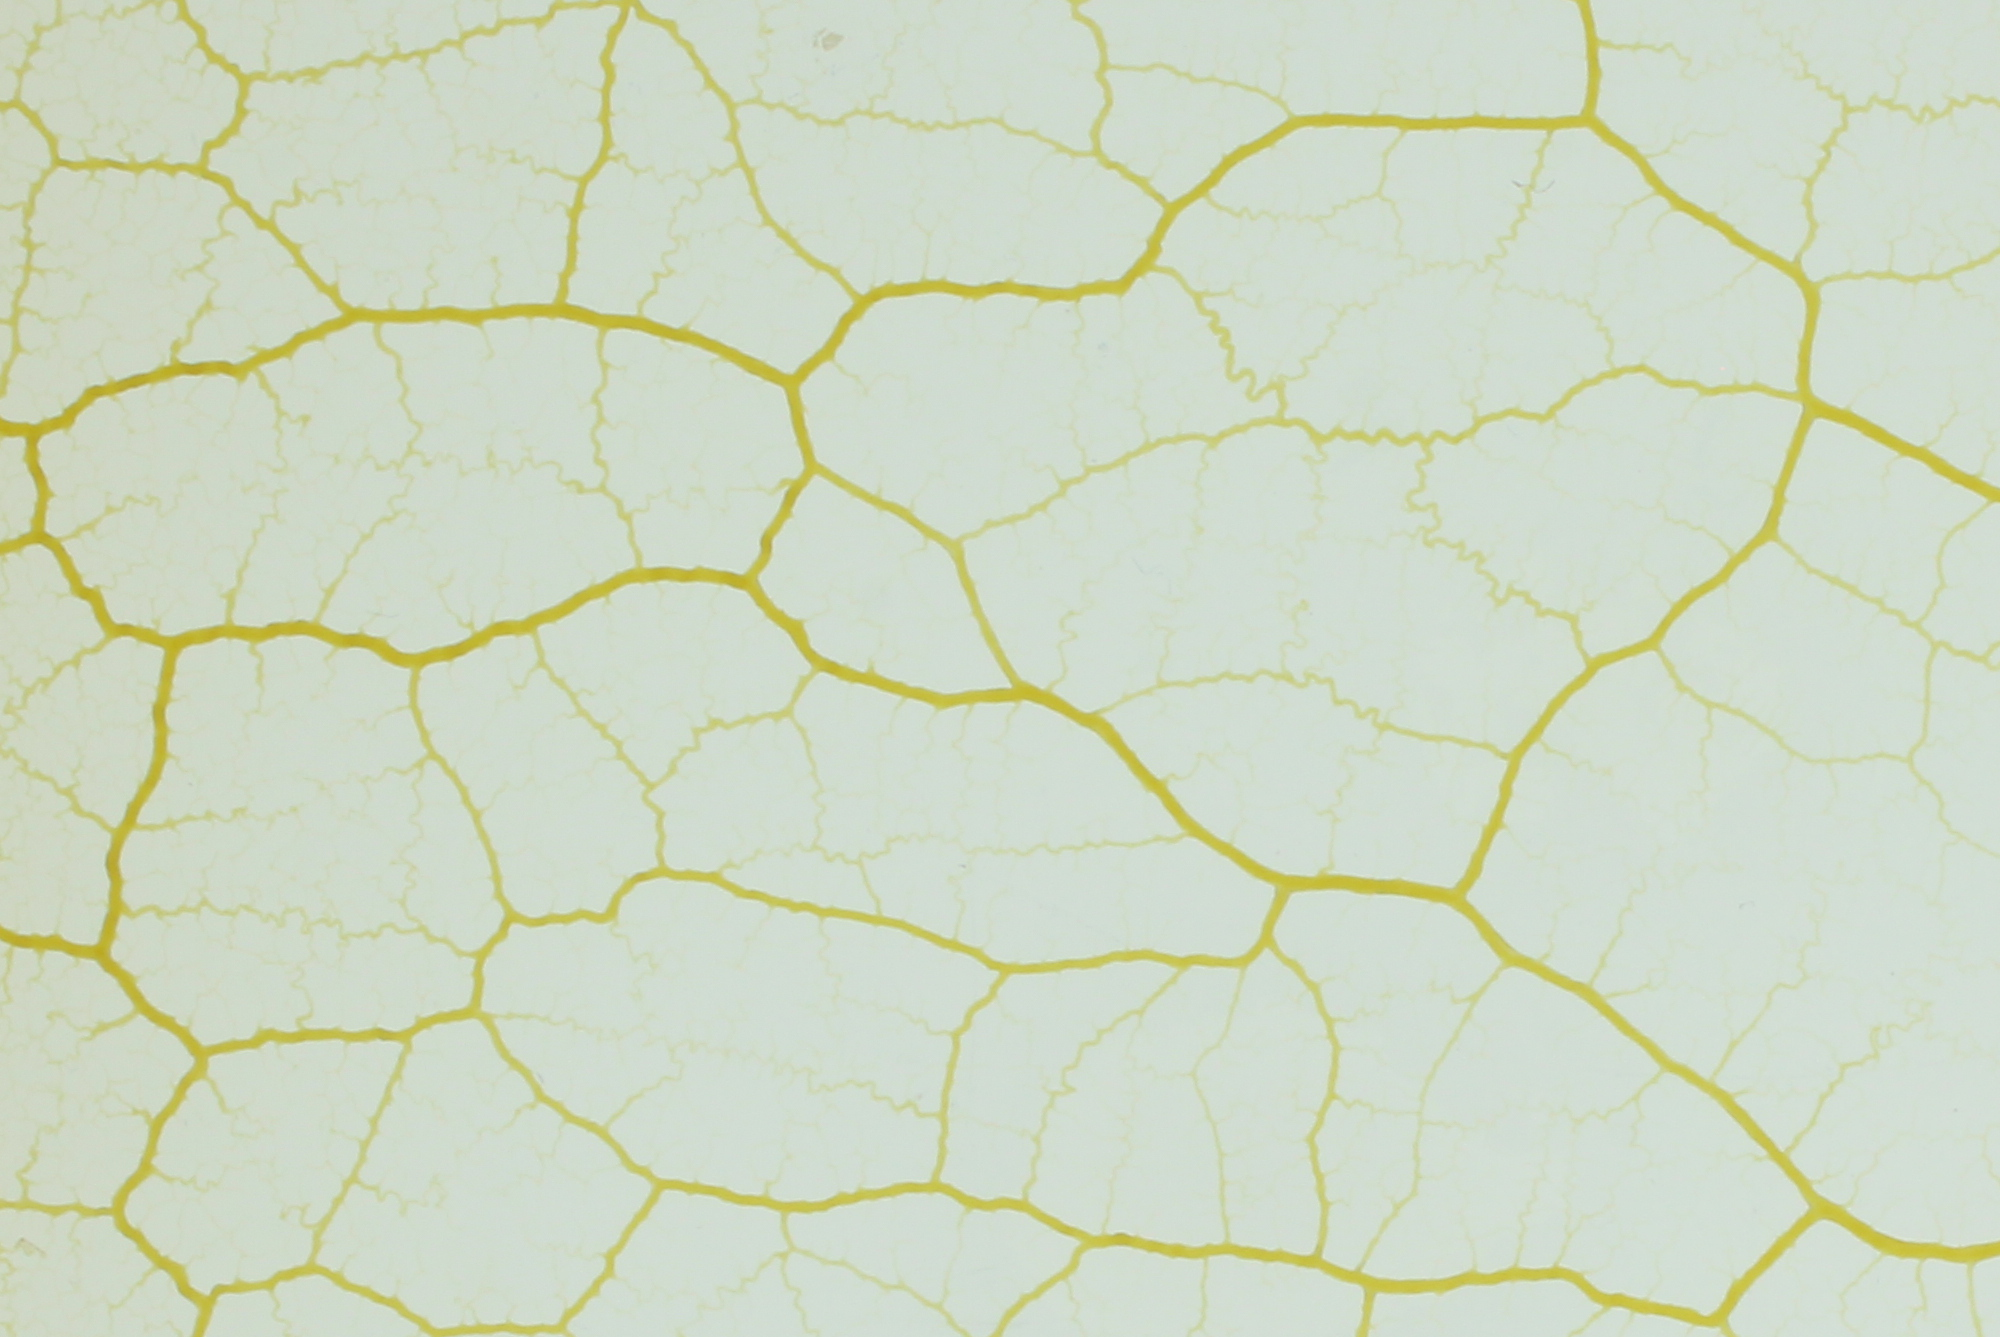
\includegraphics[width=\twoimageswide]{network.JPG}\label{fig:supporting_network}}
			\caption[Details of apical zone and supporting network]{(a) Detailed image of the apical zone being supported by thick veins. (b) A larger example of the complex vein network. Note the large cycles of thick veins. Smaller veins provide additional connections.}
			\label{fig:plasmodium_details}
		\end{figure}

		
	
		The veins themselves are approximately cylindric with vein walls consisting of a thick connected mesh of Actin and Myosin fibers. They connect to form a complex planar vein network. Within the veins protoplasmic fluid, or protoplasm for short, can freely flow back and forth. Protoplasmic flow transports cell nuclei, nutrients and various other relevant factors. \Fref{fig:plasmodium_hand_drawing} shows a schematic drawing of a macro plasmodium.

		\begin{figure}[!htb]
			\centering
			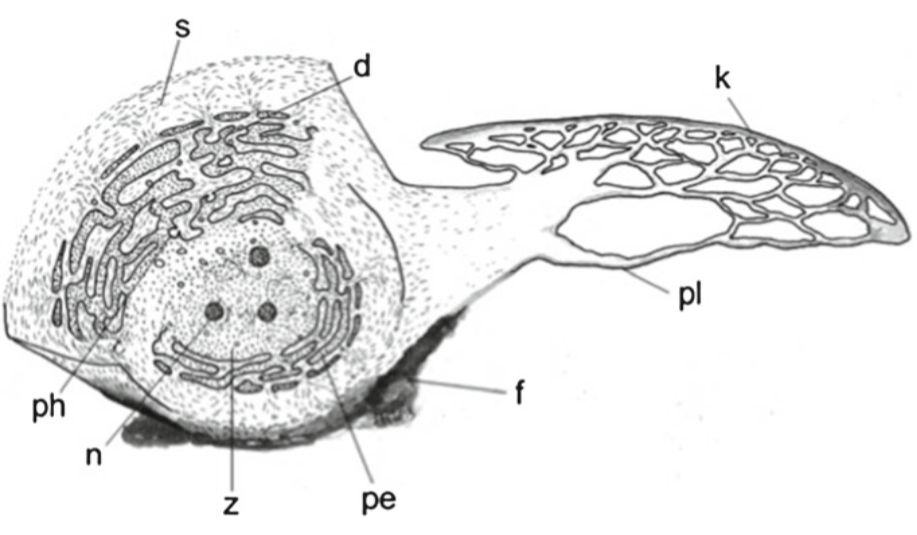
\includegraphics[width=\oneimagewide]{plasmodium_hand_drawing.png}
			\caption[Schematic drawing of the plasmodium of \P]{Schematic drawing of slime mold plasmodium with facing side sectioned and upper left section enlarged. \textbf{\texttt{k}} moving front, \textbf{\texttt{pl}} trailing plasmodial strand, \textbf{\texttt{f}} deposited material, \textbf{\texttt{s}} slime; \textbf{\texttt{d}} vacuole with deposit; \textbf{\texttt{ph}} phagocytosis vesicle; \textbf{\texttt{n}} nucleus; \textbf{\texttt{z}} central plasma; \textbf{\texttt{pe}} peripheric membrane stacks. Peristaltic contractions occur in the peripheric plasma, while the central plasma is subject to shuttle streaming. Hand-drawing by Prof.~M.~Grube, Karl-Franzens University of Graz. Reprinted with permission from~\cite{grube2016physarum}.}
			\label{fig:plasmodium_hand_drawing}
		\end{figure}

		The protoplasmic flow itself is driven by periodic cross-sectional contractions of the actin-myosin mesh forming the walls of the veins. The contractions cause a peristaltic pumping effect inducing protoplasmic streaming and net material transport. Resulting peristaltic contraction waves can be observed across the entire network inducing complex flow patterns including periodic flow arrests and reversals. Every \SI{50 \pm 5}{\second} the velocity of the protoplasmic flow streaming through a vein decays smoothly until the flow completely arrests. After one or two seconds of standstill, flow velocity quickly accelerates back to normal and the cycle proceeds. Interestingly, after most but not all arrests, the direction of flow is reversed after the flow picks up again. Protoplasmic flow exhibits enormous flow speeds of up to \SI[per-mode=symbol]{1000}{\micro\metre\per\second}\footnote{Note that $\SI{1000}{\micro\metre} = \SI{1}{\milli\metre}$. Also note that flow speeds of \SIrange[per-mode=symbol]{2}{78}{\micro\metre\per\second} known for streaming plasma in plants pale in comparison.}. It is believed that the interplay of network topology, peristaltic pumping and complex flow patterns with high flow velocity facilitates efficient transport of nutrients and signaling molecules across the entire organism. 

		In addition to enabling fluid transport, flow patterns also cause periodic pressure waves arriving at the apical zones of the organism. Each incoming wave extends the organism boundary by a small amount by pushing forward protoplasm that arrives via the vein network. This process is called shuttle streaming. Since the pressure of the streaming protoplasm is very high, material practically shoots out of the supporting veins, resulting in fan-like growing tips which can be seen along the boundary of the organism, see \Fref{fig:apical_zone}. As the advancing growing front leaves behind a network of veins, continued support for expansion is ensured.

		Given abundant food supply, \P rapidly advances a coherent and dense apical zone exploring the available space. The growing front proceeds as one large unit following an exploration strategy aptly termed \emph{phalanx}, see \Fref{fig:exploration:lab} or \Fref{fig:apical_zone}. If nutrients are scarce, however, a different strategy is employed and \P tends to grow several separate distinct growing tips, each advancing their own substantially smaller growing front. This behavior increases the odds of discovering more distant sources of nutrients. Since branches may react individually to attractants such as food, a more adaptive search is achieved. Once new food sources are secured, the organism can concentrate its movement towards them by reallocating its mass as needed. This strategy has been termed \emph{guerilla}. \Fref{fig:exploration:forest} shows a separate growing tip on the right side. The figure also hints at the fact that the plasmodium of \P can naturally interpolate between the two extreme strategies. The strategies employed by \P are reminiscent of two well know graph traversal strategies: Breadth-first and Depth-first search. In BSF, the explored region grows uniformly like a wave that expands evenly in all available directions. In contrast to that, DFS chooses one direction in order to explore it to maximum depth first. Only then does it backtrack to resolve other places ignored so far.

		Finally, we remark that the plasmodium stage of \P can be regarded as simple in terms of its biological organization because it lacks any form of brain or nervous system capable of orchestrating complex tasks such as foraging for food. The fact that the organism still displays a level of complex organized behavior sufficient to survive is one of its most fascinating features. Today it is believed that effective global organization emerges from the delicate interplay of local effects such as periodic contractions, topological dynamics and the integration of environmental signals. Shedding light on the details of these dynamics remains one of the major challenges in \P research.

		\FloatBarrier

	\subsection{Overview of Research Focused on P.~Polycephalum}

		\P develops exceptionally well when cultured in the lab which makes it an ideal subject for scientific studies. Significant research activity in the beginning of the latter half of the 20th century explored the life cycle of \P and described the morphology and physiology of its various stages for the first time. Culturing procedures as well as genetic and molecular techniques were developed which allowed a detailed study of its mitotic cycle, cellular motility, differentiation and many other questions of biological interest. Although interest in \P was at first exclusively fueled by general questions of biology, a wider scientific community soon began to appreciate the value of \P as a multi-potent model system that could be controlled and studied effectively. Within a short period \P became a core experimental platform, driving a variety of different research efforts. The study of cell motility is particularly noteworthy in this context. Relevant reviews dating from the 1980s can be found in~\cite{dove1980growth, aldrich2012cell,sauer1982developmental,Sauer1986}.

		After a period of intense research up to the 1980s, the remainder of the century saw a general decline in interest related to \P. It should not end until the beginning of the 21th century, when exciting new question surrounding the networks formed by the plasmodium of \P arose\footnote{Some members of the research community today have been humorously referring to these events as ``the second coming'' of \P.}. In particular, it was shown that the vein networks formed by the plasmodium of \P exhibit highly localized dynamic oscillatory behavior and a capability to adaptively change their topology. Together with its remarkable chemotactic abilities, these properties play a key role in the foraging behavior of \P. Despite the lack of any centralized control, they enable the organism to act as an organized unit in order to establish robust and effective vein networks connecting a potentially large set of spatially distributed food sources. 

		In a similar context, the vein network established by \P has been shown experimentally to mimic man-made transportation networks such as railway systems or highways~\cite{tero2010rules,Tero2006115,Nakagaki20041}. Furthermore, it has been demonstrated that the plasmodium of \P can establish the shortest path between a pair of food sources placed in a maze~\cite{nakagaki2000intelligence}. These astounding feats received major interest amongst scientists of many disciplines and simultaneously earned \P a place in the perception of the general public. Within a short period of time, \P became the focus of diverse interdisciplinary research efforts, engaging biologists, physicists and computer scientists alike. The renewed multi-disciplinary interest lead to a resurgence of research in \P that can be observed to this day. For a rare, more recent review, and various recent results see~\cite{ueda2005intelligent} and~\cite{takamatsu2009environment,shirakawa2007emergence,alim2013random,Tero2007553,nakagaki2004obtaining}. Please note that this selection represents a fairly limited part of current research on \P. In fact, it is focused on results revolving around the network forming plasmodium stage of \P which are relevant in the context of this thesis.

		\FloatBarrier
